\documentclass[xcolor=dvipsnames]{beamer}
%\documentclass[handout,xcolor=dvipsnames,pdftex,hyperref={colorlinks=false}]{beamer}

% == Packages
\usepackage{xcolor}
\usepackage{graphicx}
\graphicspath{{./}{figures/}}
\usepackage{fancybox}
\usepackage{hyperref}
\usepackage{amsmath,amssymb,amsfonts,bm}
\usepackage{wasysym}
\usepackage{colortbl}
\usepackage[english]{babel}
\usepackage{times}
\usepackage{multirow}
\usepackage{rotating}
\usepackage{latexsym}
\usepackage{ulem}
\usepackage{booktabs}
\usepackage{appendixnumberbeamer}
\usepackage{natbib}
\usepackage{tikz}
\usepackage{comment}

\usetikzlibrary{positioning,arrows.meta}

\usetheme{Warsaw}
\usepackage{helvet}
\definecolor{someblue}{rgb}{0,.1,0.8}
\definecolor{dgreen}{rgb}{0,.6,0.8}
\useoutertheme{infolines}

% == Typesetting helpers
\newcommand\spacingset[1]{\renewcommand{\baselinestretch}{#1}\small\normalsize}
\renewcommand\r{\right}
\renewcommand\l{\left}
\newcommand\makegaps{\addtolength{\itemsep}{.25\baselineskip}}
\newcommand\smallunskip{\vspace{-.25\baselineskip}}
\newcommand\medunskip{\vspace{-.5\baselineskip}}
\newcommand\bigunskip{\vspace{-\baselineskip}}

% == Math / stats
\renewcommand{\epsilon}{\varepsilon}
\newcommand\E{\mathbb{E}}
\newcommand\V{\mathbb{V}}
\newcommand\Y{{\bm Y}}
\newcommand\X{{\bm X}}
\newcommand\D{{\bm D}}
\newcommand\eps{{\bm\varepsilon}}
\newcommand\indep{\protect\mathpalette{\protect\independenT}{\perp}}
\def\independenT#1#2{\mathrel{\rlap{$#1#2$}\mkern2mu{#1#2}}}
\newcommand{\Var}{\mathrm{Var}}
\DeclareMathOperator{\SCQE}{SCQE}

\newtheorem{assumption}{Assumption}

\AtBeginSection[]
{
  \begin{frame}<beamer>
    \frametitle{Outline}
    \tableofcontents[currentsection]
  \end{frame}
}

\title[SCQE]{Safe inference and the stability-controlled quasi-experiment (SCQE)}
\subtitle[ ]{PS200C, Spring 2026}
\author[Hazlett]{Chad Hazlett}
\institute[UCLA]{UCLA\\[1ex]\texttt{chazlett@ucla.edu}}
\date{}

\begin{document}

\subject{Talks}

% ============================================================
\begin{frame}
  \titlepage
\end{frame}

\begin{frame}{Roadmap}
\begin{enumerate}\makegaps
  \item Motivation: ``safe inference'' as a posture
  \item The SCQE idea and identification
  \item Applications: dexamethasone, HCQ, remdesivir
  \item Relationship to other strategies (DID, SOO$+$sensitivity)
  \item Wrap-up
\end{enumerate}
\end{frame}

% ============================================================
\section{Motivation: safe inference}
% ============================================================

\begin{frame}{Motivation}
\onslide<1-> Many high-stakes treatments get rolled out, taken, or assigned \emph{without} randomization.\\
\medskip
For example: in the early pandemic, many people were given unproven therapies outside of RCTs. \textbf{What could we have learned from those experiences?}\\
\bigskip
\onslide<2-> \textcolor{blue}{Reaction 1}: ``If it isn't an RCT, it is rubbish.''\\
\small
\begin{itemize}
\item Healthy starting point...point estimate cannot be trusted...but going beyond the heuristic you might find reliable information.
\end{itemize}
\medskip
\normalsize
\onslide<3-> \textcolor{blue}{Reaction 2}: ``Make a heroic assumption, call the estimate \emph{suggestive}.''\\
\small
\begin{itemize}
  \item Covariate adjustment $+$ no-unobserved-confounders is the classic case, but the same goes for IV, DID, synth, etc.
  \item Even calling the results ``suggestive'' is dangerous... helpful treatments may look harmful, vice versa.
\end{itemize}
\end{frame}

\begin{frame}{An alternative: safe inference}
\onslide<1-> \textcolor{blue}{Safe inference}: partial identification $+$ sensitivity analysis.\\
\bigskip
\small
\begin{itemize}\makegaps
  \item<2-> Pick an identification strategy whose \textbf{assumptions you are equipped to argue about}.
  \item<3-> Argue what \textbf{bounds} you can defend on those assumptions, see what conclusion they buy you.
  \item<4-> Report ranges of estimates indexed by the assumption, not a single point estimate that hides the assumption.
\end{itemize}
\bigskip
\onslide<5-> We did something of this kind with SOO + sensitivity. \\
\medskip
\onslide<6-> Today: a different identification strategy, designed to be argued about transparently.
\end{frame}

% ============================================================
\section{The SCQE idea and identification}
% ============================================================

\begin{frame}{The stability-controlled quasi-experiment (SCQE)}
\medskip
\onslide<1-> Example: COVID-19 patients admitted to a hospital in Feb--Mar 2020.\\
\small
\begin{itemize}
    \item Of patients admitted in February, 0\% got dexamethasone
    \item Of patients admitted in March, 30\% (very non-randomly) received it
\end{itemize}
\bigskip
\normalsize
\onslide<2-> Ask yourself, absent this treatment how much could the mortality rate change from one month to the next?  I.e. the ``baseline trend''. \\

\[\textcolor{blue}{\delta} \equiv \E[Y(0)|T=1] - \E[Y(0)|T=0]  \]

\bigskip
\onslide<3->  \textcolor{blue}{This baseline trend $\delta$ is the \emph{only} assumption required to get the ATT.}

\end{frame}

\begin{frame}{SCQE: Arguments about $\delta$}
We'll come back to this in practice but to set the stage:  You don't know $\delta$ and it doesn't live in the data. But, you can reason about it through:
\small
\begin{itemize}
\item<2-> Hard bounds (mortality rate between 0 and 1)
\item<3-> Reasonable (disputable) bounds: mortality almost surely didn't double, or halve, from one month to the next; if it had we would know...
\item<4-> Informed bounds: based on observed changes in patient characteristics, other treatments, and expert judgment, you might guess that mortality (absent dexamethasone) likely dropped by...
\end{itemize}
\bigskip
\normalsize
\onslide<5-> Don't worry we won't need point values for $\delta$...there will be good uses for (i) defensible ranges, (ii) unbelievable ranges, or even just (iii) ranges where you cannot be sure either way...all will contribute to characterizing what we can(not) conclude. 
% Instead you can either:\\
% \begin{itemize}
% \item Argue for an \textit{ex ante} defensible range of $\delta$ values, and report the corresponding range of estimates. Or,
% \item Reveal ``what $\delta$ you'd have to believe'' to defend some research conclusion, which helps reveal what we shouldn't be claiming at all, or with certainty.
% \end{itemize}
\end{frame}

\begin{frame}{How does $\delta$+data tell you the ATT?}
\begin{columns}[T]
\begin{column}{0.45\textwidth}
\vspace{0.5em}
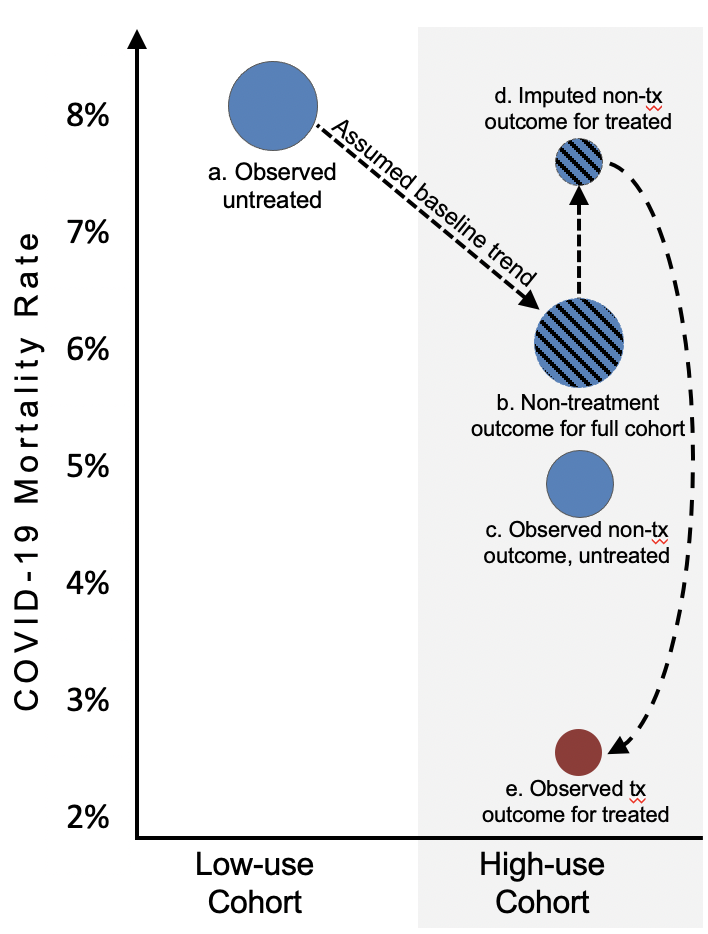
\includegraphics[width=\textwidth]{SCQEconcept.png}
\end{column}
\begin{column}{0.55\textwidth}
\footnotesize
\begin{itemize}\makegaps
\item<2-> We observe (a), $\E[Y(0)|T=0]$. For a postulated $\delta$, you get out (postulated) $\E[Y(0)|T=1]$ (b). 
\item<3-> Meanwhile in later cohort, you observe $\E[Y(0)|T=1,D=0]$ (c). 
\item<4-> Then you can back out $\E[Y(0)|T=1,D=1]$ (d). 
\item<5-> We observe $\E[Y(1)|T=1,D=1]$ (e), and that minus (d) is the ATT.
\end{itemize}
\end{column}
\end{columns}
\end{frame}

\begin{frame}{Mathified,}
Define the change in non-treatment average outcomes,\\
\footnotesize
\begin{align}\label{eq:delta}
\delta & \equiv \E[Y(0)| T=1]-\E[Y(0)|T=0].
\end{align}
\normalsize
\onslide<2-> By LIE,
\footnotesize
\begin{align*}
\color{Green}{\E[Y(0)|T=1]} &= \textcolor{blue}{\E[Y(0)|T=1,D=1]}\pi_1 + \E[Y(0)|T=1,D=0](1-\pi_1)
\end{align*}
\normalsize
So we have
\footnotesize
\begin{align}
\color{Green}{\E[Y(0)|T=0] + \delta} &= \textcolor{blue}{\E[Y(0)|T=1,D=1]}\pi_1 + \E[Y(0)|T=1,D=0](1-\pi_1) \\
\textcolor{blue}{\E[Y(0)|D=1, T=1]} &= \frac{\E[Y|T=0] - \E[Y| D=0, T=1](1-\pi_1) + \delta }{\pi_1 } \label{missingPO}
\end{align}
\normalsize
\onslide<3-> So if you want the ATT at $T=1$,
\footnotesize
\begin{align}
    ATT &\equiv \E[Y(1)|D=1, T=1] - \textcolor{blue}{ \E[Y(0)|D=1, T=1]} \nonumber \\
    &=  \E[Y|D=1, T=1] - \left(\frac{\E[Y|T=0] - \E[Y| D=0, T=1] (1-\pi_1)  + \delta}{\pi_1 }\right). \label{est:ATT}
\end{align}
\end{frame}

\begin{frame}{Some details}
\small
\begin{itemize}
\item<1-> Works the same way when there are treatment-takers in both periods --- what you need is a \textbf{big change in treatment probability}. (You then get a LATE-like quantity rather than the ATT.)
\bigskip
\item<2-> The two ``cohorts'' could be different facilities, eras, or sites --- whatever defines a sharp shift in treatment probability, as long as you can reason about non-treatment outcome differences between them.
\bigskip
\item<3-> In fact you could do this with just one study cohort, and any guess of $\E[Y(0) \mid \text{your study sample}]$ (more soon)
\end{itemize}
\end{frame}

\begin{frame}{Connection to IV: time as the instrument}
\onslide<1-> Cohort/time is like an encouragement to treatment:
\small
\begin{itemize}
\item<2-> If no one is treated in the first cohort, you have one-way non-compliance (no always-takers), so the complier-ATE is just the ATT.
\item<3-> \textbf{But}: the exclusion restriction is \emph{not} expected to hold here. Time affects mortality through many other channels... that is what $\delta$ is about!
\item<4-> The math effectively subtracts the exclusion restriction violation off, 
\end{itemize}
\bigskip
\normalsize
\onslide<5-> Concretely: define a pseudo-outcome $\tilde Y_i \equiv Y_i - \delta T_i$. Then under SCQE assumptions $\tilde Y_i(0) \indep T_i$, and the Wald estimator gives:
\footnotesize
\[
ATT \;=\; \frac{\E[Y|T=1] - \E[Y|T=0] - \delta}{\pi_1}.
\]
...which is just a (simpler looking) rearrangement of the SCQE estimator in \eqref{est:ATT}.
\end{frame}

% ============================================================
\section{Applications}
% ============================================================

\begin{frame}{Worked example: dexamethasone for COVID-19}
\textbf{Cohorts}:\footnote{\scriptsize Wulf, Hazlett, Hill, Chiang, Goodman-Meza, Pasaniuc, Arah, Erlandson, Montague.
``Safe inference outside of randomized trials: Application of the stability-controlled quasi-experiment to the effects of three COVID-19 therapies.''
\emph{Observational Studies} 11(3), 2025, 301--330.}
\small
\begin{itemize}
\item ``Low-use'' (first) cohort: days 44--101, \textbf{5.7\%} took dexamethasone
\item ``High-use'' (second) cohort:  days 102--200, \textbf{46\%} took dexamethasone
\end{itemize}
\bigskip
\normalsize
\onslide<2-> \textbf{Outcome: 14-day mortality}
\small
\begin{itemize}
\item \textbf{10.9\%} in the low-use (first) cohort
\item \textbf{5.4\%} in the high-use (second) cohort
\end{itemize}
\bigskip
\normalsize
\onslide<3-> On its surface: big uptick in treatment, big drop in mortality...promising but could it just be the \emph{baseline trend}?
\end{frame}

\begin{frame}{Dexamethasone: $\delta$ considerations}
\footnotesize
\onslide<1-> Before looking at the SCQE results, let's think about where $\delta$ might be.\\
\medskip
\onslide<1-> \textbf{Baseline characteristics.} High-use cohort had \emph{fewer} ICU admissions, ventilator use, skilled-care admits within 24h --- all consistent with a drop in baseline mortality.\\
\medskip
\onslide<2-> \textbf{Other therapies.} Higher remdesivir use in the high-use cohort (12\% vs. 27\%). Could reduce risk; unknown at the time.\\
\medskip
\onslide<3-> \textbf{Modeled mortality risk on observables.} Predicted baseline mortality fell by 1.3--2.1pp.\\
\medskip
\onslide<4-> \textbf{Expert judgement.} Physicians on the team expected baseline mortality to drop with generally improving practice over this period.\\
\medskip
\onslide<5->
\begin{quote}\small
``All lines of evidence suggest a possible drop in baseline mortality. Taking these considerations collectively, and maintaining a conservative attitude, we postulated that a plausible range for the baseline trend ranged from \emph{no change} to a reduction of up to 5pp ($-46\%$).''
\end{quote}
\end{frame}

\begin{frame}{Dexamethasone: results}
\begin{figure}[!t]
    \centering
    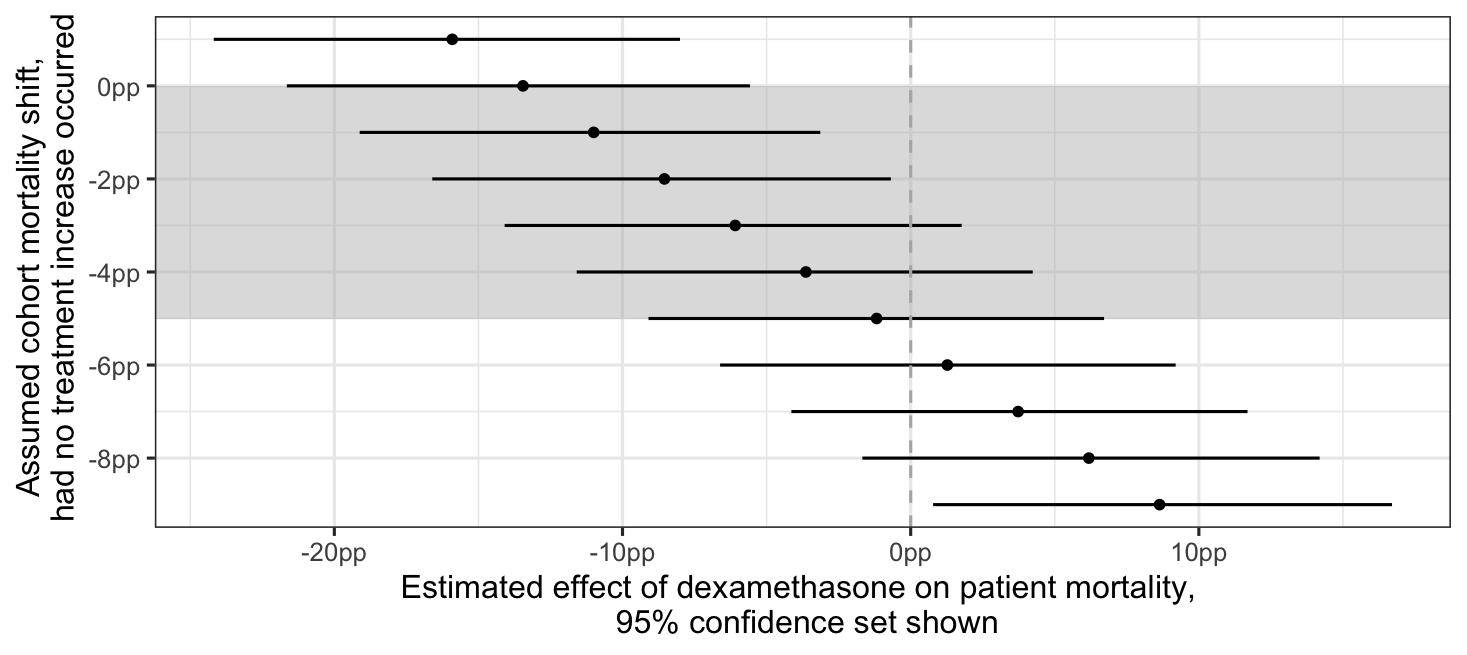
\includegraphics[width=0.78\textwidth]{scqe_plot_dex_range.png}
\end{figure}
\footnotesize
\begin{itemize}
\item<1-> Beneficial ($p<0.05$) if baseline mortality increased, flat, or fell by up to 2.3pp ($-21\%$)
\item<2-> Non-harmful point estimate until a drop of 5pp ($-46\%$)
\item<3-> Harmful ($p<0.05$) only if baseline mortality fell by 6.8pp ($-93\%$), leaving mortality of just 0.4\%
\end{itemize}
\end{frame}

\begin{frame}{Dexamethasone: what we concluded}
\begin{quote}
``We consider [the drop in baseline required to support a harmful effect] to be extremely unlikely, particularly without a known cause that escaped the attention of physicians on the team and does not appear in the observable differences in cohorts.''
\end{quote}
\medskip
\onslide<2->
\begin{quote}
    ``Thus, we have considerable confidence that dexamethasone was at least directionally, and possibly statistically significantly beneficial, and that it was not significantly harmful.''
\end{quote}
\medskip
\onslide<3-> \small Consistent with the eventual results of the RECOVERY-trial.
\end{frame}

\begin{frame}{Hydroxychloroquine (HCQ): results}
\small
\onslide<1-> \textbf{Cohort shift:} 36\% HCQ use in high-use early cohort $\to$ 2.9\% in low-use cohort. Mortality 11.6\% $\to$ 8.6\%.\\
\medskip
\onslide<2-> Observables/ expertise suggested: ``a wide range of baseline trends are possible, from +1pp to $-4.5$pp.''\\
\bigskip
\begin{center}
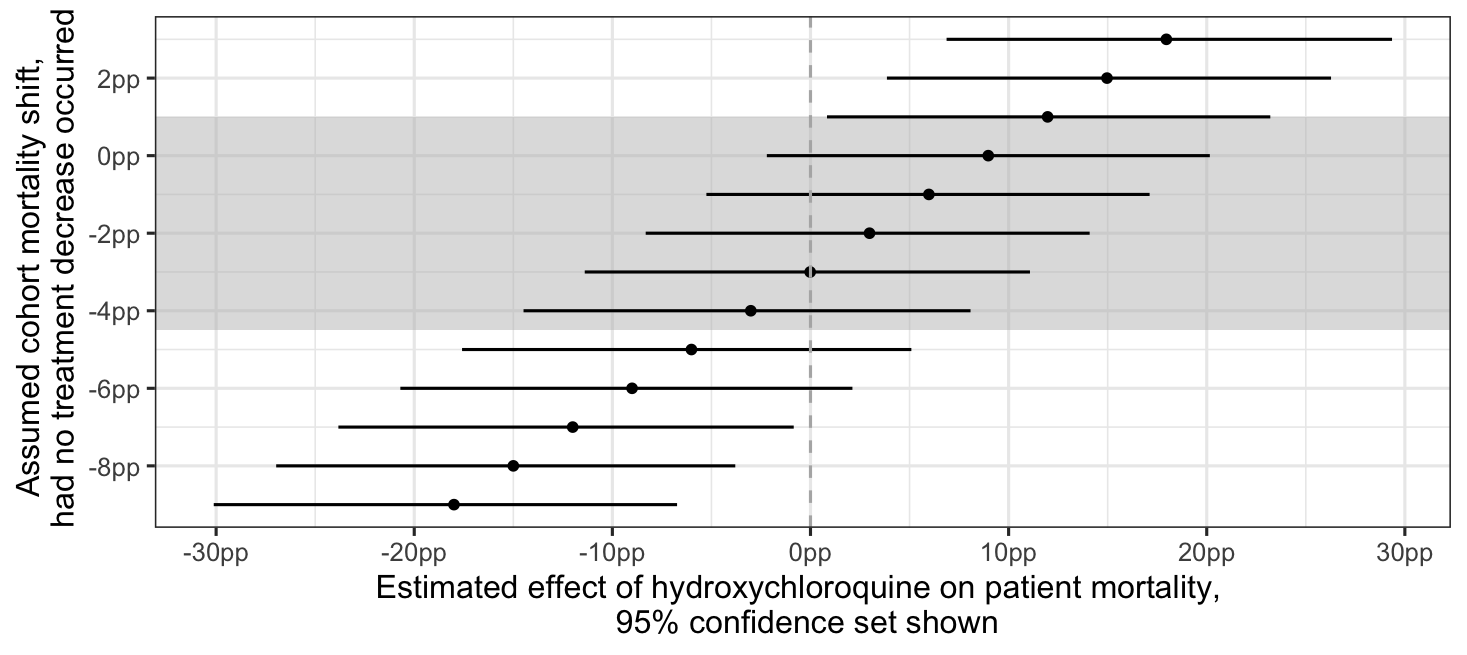
\includegraphics[width=.65\textwidth]{scqe_plot_hcq_range.png}
\end{center}
\footnotesize
\onslide<3-> Wide plausible range of $\delta$ in which you would conclude HCQ was \textbf{harmful}.\\
\smallskip
\onslide<4-> Sig. harmful if baseline mortality worsened by even 0.7pp. \\
\smallskip
\onslide<5-> Sig. beneficial only if baseline improved by $\geq$6.7pp ($-46\%$): not credible.
\end{frame}


\begin{frame}{Remdesivir: results}
\small
\onslide<1-> \textbf{Cohort:} 0\% remdesivir use in no-use cohort $\to$ 31.3\% in high-use cohort. Mortality 24.5\% $\to$ 13.3\%.\\
\medskip
\onslide<2-> Observables and clinical judgment: plausible range $\delta \in [+2.5\text{pp}, -15\text{pp}]$.\\
\begin{center}
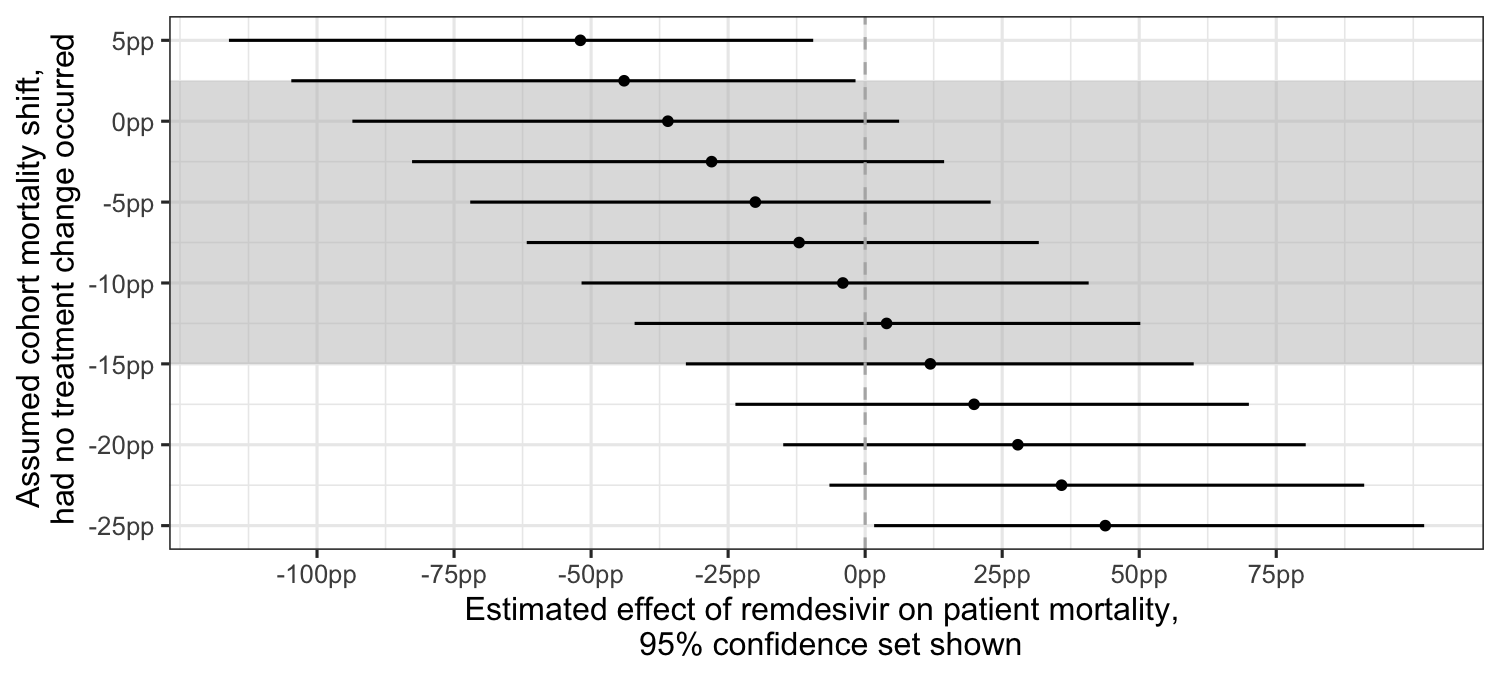
\includegraphics[width=.65\textwidth]{scqe_plot_rem_range.png}
\end{center}
\footnotesize
\onslide<3-> While benefit is plausible, cannot rule out harm (on point estimates). \\
\smallskip
\onslide<4-> Can rule out statistically significant harm -- would imply $0\%$ counterfactual mortality. 
\end{frame}

\begin{frame}{Conclusions}
\small
\begin{itemize}\makegaps
  \item<1-> \textbf{Dexamethasone:} likely beneficial or null. Harm would require an implausibly large drop in baseline mortality.
  \item<2-> \textbf{HCQ:} Could be (sig.) harmful with small positive $\delta$. Sig. benefit would require larger drop than deemed plausible.
  \item<3-> \textbf{Remdesivir:} sig. benefit is plausible but so is harmful (point) estimate. Not sig. harmful.
\end{itemize}
\bigskip
\onslide<4-> \textbf{If you had to decide what to do,} you'd have some guidance -- it would take insane assumptions to believe HCQ will help, whereas dexamethasone possibly could; neither dexamethasone nor remdesivir can reasonably be significantly harmful, but HCQ can be.\\
\bigskip
\onslide<5-> Not precise, but a long way from either ``we can't say anything without an RCT'' or ``the observational study is our best guess.'' 
\end{frame}

% ============================================================
\section{Relationship to other strategies}
% ============================================================

\begin{frame}{Relationship to DID}
\textbf{Case 1:} You can't do DID at all.\\
\small
\begin{itemize}
    \item DID requires labeling units pre-treatment as ``would-be-treated'' vs. control.
    \item Impossible in cases like this -- you cannot label patients in the first cohort as ``would-be treated''.
\end{itemize}
\medskip
\normalsize
\onslide<2-> \textbf{Case 2:} You can define those groups.\\
\small
\begin{itemize}
    \item Parallel trends = the two groups share a trend in $\E[Y(0)]$.
    \item  Suppose you just look at change in mean outcomes in the control group, and you assume that is exactly $\delta$.  
    \item That is DID! So \textcolor{blue}{DID is a special case of SCQE}, with a particular assumption about $\delta$.
    \item SCQE shows DID as one estimate in a \emph{range}, indexed by $\delta$.
\end{itemize}
\end{frame}

\begin{frame}{Relationship to covariate adjustment $+$ sensitivity}
\small
\onslide<1-> What does SCQE reveal that a sensitivity-analyzed covariate-adjustment analysis wouldn't?\\
\bigskip
\onslide<2-> Direct point-estimate comparison is not meaningful here.\\
\bigskip
\onslide<3-> Instead, compare what \emph{conclusions} you could defend through each:
\begin{itemize}
\item<4-> Across these COVID applications, unobserved confounding explaining $\approx$18\% of residual variance in treatment \emph{and} outcome would suffice to flip the significance of any conclusion under covariate adjustment.
\item<5-> We can't really rule that out...so we can't rule out any conclusions via SOO+sensitivity.
\end{itemize}
\bigskip
\onslide<6-> Different assumptions offer different leverage... use what works.
\end{frame}

\begin{comment}
% ============================================================
\section{One-cohort SCQE: external control arms}
% ============================================================

\begin{frame}{What if there's only one cohort?}
\onslide<1-> So far: two cohorts of patients with different treatment rates.\\
\medskip
\onslide<2-> But many real settings have effectively \emph{one} cohort:\\
\small
\begin{itemize}
  \item Single-arm trials (no internal control)
  \item Trials with an external control arm (ECA) drawn from EHR / prior trials / registry
  \item Trials that started randomized but lost the comparison (e.g., heavy crossover)
\end{itemize}
\bigskip
\normalsize
\onslide<3-> SCQE applies essentially unchanged, with one reinterpretation: \\
\medskip
\onslide<4-> \begin{center}
\textcolor{blue}{$\delta$ is now the gap in $\E[Y(0)]$ between your trial cohort and your external comparison source.}
\end{center}
\end{frame}

\begin{frame}{One-cohort form}
\onslide<1-> All-treated cohort (so $\pi_1 = 1$, $\E[Y|T=1] = \E[Y|D=1,T=1]$). External source supplies $\E[Y|T=0]$.\\
\medskip
\onslide<2-> Then the ATT formula collapses:
\footnotesize
\[
ATT \;=\; \E[Y|D=1, T=1] \;-\; \bigl( \E[Y|T=0] + \delta \bigr).
\]
\normalsize
\medskip
\small
\onslide<3-> What $\delta$ means now:
\begin{itemize}
\item Differences in eligibility, geography, era, case mix between trial and external source
\item Anything that would shift untreated outcomes in your cohort vs. theirs
\end{itemize}
\medskip
\onslide<4-> \textbf{This is the partial-ID version of an external control arm.}\\
\smallskip
Instead of asserting the external cohort is comparable, you ask: how much non-comparability could there be, and what range of conclusions does that buy?
\end{frame}

\begin{frame}{Application: glioblastoma multiforme (GBM)\footnote{\scriptsize Ongoing work; results below are illustrative pending finalized analysis.}}
\small
\onslide<1-> \textbf{Setting.} A Phase III trial of DCVax-L, a personalized dendritic cell vaccine for newly-diagnosed GBM.
\begin{itemize}
\item Trial suffered substantial crossover; standard analysis rendered uninformative.
\item Analysis was reframed against an external control arm (ECA) from contemporaneous patients.
\item Reviewers responded heuristically: ``crossover $+$ external control $\Rightarrow$ findings dismissed.''
\end{itemize}
\bigskip
\onslide<2-> \textbf{Why this setting suits SCQE.}\\
GBM has a \emph{well-characterized natural history}: median survival, 2-year mortality, and prognostic markers are highly predictable absent treatment. So the comparability assumption $\delta$ is something the field actually can argue about.
\bigskip
\onslide<3-> \textbf{The SCQE question.} For what range of $\delta$ (gap in 2-year mortality, trial cohort vs. ECA, absent treatment) do we conclude DCVax-L beneficial / harmful / indeterminate?
\end{frame}

\begin{frame}{GBM, illustrative numbers}
\small
\onslide<1-> (Numbers below are placeholders pending confirmation against the finalized analysis.)\\
\medskip
\textbf{Cohorts:}
\begin{itemize}
\item Trial cohort (all-treated for SCQE purposes; $\pi_1 = 1$): $n \approx 230$, 2-year mortality $\approx 55\%$.
\item External control source: 2-year mortality $\approx 65\%$.
\end{itemize}
\medskip
\onslide<2-> \textbf{$\delta$ considerations:}
\begin{itemize}
\item Trial eligibility likely tilts toward healthier patients $\Rightarrow$ baseline mortality in trial cohort plausibly \emph{lower} than ECA, so $\delta < 0$.
\item Domain experts can put a range on this from known prognostic differences.
\item Conservative plausible range: $\delta \in [-15\text{pp}, +5\text{pp}]$.
\end{itemize}
\medskip
\onslide<3-> Naive comparison ($\delta=0$) implies $ATT \approx -10$pp. SCQE then shows what survives at each end of the plausible range.
\end{frame}

\begin{frame}{GBM: what the partial-ID answer looks like}
\small
\onslide<1-> (Schematic; populate with the actual SCQE plot once the analysis is finalized.)\\
\medskip
\textbf{The kind of conclusion SCQE produces here:}
\begin{itemize}\makegaps
  \item<2-> If the trial cohort was up to (say) 10pp healthier than the ECA absent treatment, DCVax-L still appears beneficial.
  \item<3-> If the trial cohort was 15pp healthier --- the conservative edge of the plausible range --- the effect is null.
  \item<4-> A harmful conclusion would require the trial cohort to be \emph{$>$15pp healthier} on baseline mortality than the ECA. Reviewers can be asked to defend such a claim explicitly.
\end{itemize}
\bigskip
\onslide<5-> \textcolor{blue}{This is what the ``external control arm'' question \emph{should} look like: an explicit range of conclusions indexed by an explicit comparability assumption, rather than a yes/no on whether the ECA was ``valid.''}
\end{frame}
\end{comment}
% ============================================================
\section{Wrap-up}
% ============================================================

\begin{frame}{Software}
\onslide<1-> \textbf{R package} \texttt{scqe}: \url{https://github.com/chadhazlett/scqe}\\
\small
\begin{itemize}
\item Two-cohort and one-cohort modes (full data or summary stats)
\item ATT estimates and CIs over a range of $\delta$
\item Anderson--Rubin intervals and block-bootstrap CIs
\end{itemize}
\bigskip
\normalsize
\onslide<2-> \textbf{Browser calculator}: \url{https://chadhazlett.com/scqe-app/}\\
\small
\begin{itemize}
\item Type in cohort-wise summary stats, get the SCQE plot back
\item Both two-cohort and one-cohort tabs
\item Includes the dexamethasone worked example as a built-in case
\end{itemize}
\bigskip
\normalsize
\onslide<3-> You can plug in just cohort-by-treated numbers; doesn't require individual data.. 
\end{frame}

\begin{frame}{Where to use SCQE}
\small
\onslide<1-> \textbf{Medicine:}
\begin{itemize}
\item While we wait for RCTs --- present observational results in ways that prevent over-confidence
\item Therapies unlikely to be tested in trials
\item Post-approval real-world effectiveness, with different populations / protocols than trials
\item Prospective observational designs aimed at \emph{reducing} $\delta$
\end{itemize}
\bigskip
\onslide<2-> \textbf{Outside medicine}: anywhere there's a sharp change in treatment likelihood and you can't lean on no-confounding or parallel trends:
\begin{itemize}
 \item rolling out a new feature people adopt by choice
 \item effects of new classes / training programs / curricula opted into
 \item media or messaging that people consume without randomization
 \end{itemize}
\end{frame}

\begin{frame}{Takeaways}
\onslide<1-> Safe inference $=$ extract what you can with assumptions you can defend, instead of selling false certainty around a point estimate.\\
\bigskip
\small
\begin{itemize}\makegaps
\item<2-> SCQE: \emph{one} assumption, $\delta$ (the baseline trend), out in the open.
\item<3-> Different ID strategies expose different assumptions to argument --- \textcolor{blue}{use what you've got.}
\item<4-> SCQE can do work where DID and IV can't (no labeled control group, no clean exclusion).
\item<5-> The one-cohort form gives you a partial-ID treatment of external control arms.
\item<6-> Comfort with partial identification takes practice. Reporting ranges instead of points is the point.
\end{itemize}
\end{frame}

% ============================================================
\appendix
% ============================================================

\begin{frame}{Appendix: inference}
\small
Consider the regression using the pseudo-outcome $\tilde Y_i = Y_i - \delta T_i$:
\[
    \tilde{Y}_i = \beta_0 + \beta_{\SCQE} D_i + \mu_i,
\]
where $\beta_{\SCQE}$ is the SCQE estimate.\\
\medskip
\onslide<2-> Under spherical errors,
\footnotesize
\[
\widehat{SE}(\hat\beta_{\SCQE}) = \frac{\hat\sigma_\mu}{\sqrt{N}\,\hat\rho_{D,T}\,\hat\sigma_D},
\]
\normalsize\small
where $\hat\rho_{D,T}$ is the sample correlation of treatment and time indicators.\\
\medskip
\onslide<3-> More generally use the IV sandwich:
\footnotesize
\[
  \widehat{Var}(\hat\beta_{\SCQE}) = (\mathbf{Z}^\top \mathbf{D})^{-1}\mathbf{Z}^\top \hat{\mathbf{\Sigma}} \mathbf{Z}(\mathbf{Z}^\top \mathbf{D})^{-1}
\]
\normalsize\small
with $\mathbf{Z} = [1\ T]$, $\mathbf{D} = [1\ D]$, and $\hat{\mathbf{\Sigma}}$ a consistent estimator for $\Var(\mu)$ (e.g. HC2).\\
\medskip
\onslide<4-> \textbf{Alternatives in the package:} Anderson--Rubin intervals (no weak-instrument concerns), block-bootstrap over clinics for cluster-robust inference.
\end{frame}

\end{document}
